\subsection{Load Cell}

	The load cell is a transducer formed by strain gauges. Thoose are devices which their electrical resistance varies proportionally to their distension. Distension is a quantification of the deformation of a body, it can also be defined as a fractional change of the body of a body. Distension may be negative (compression) or positive (traction).

	\begin{figure}[htbp]
		\centering
			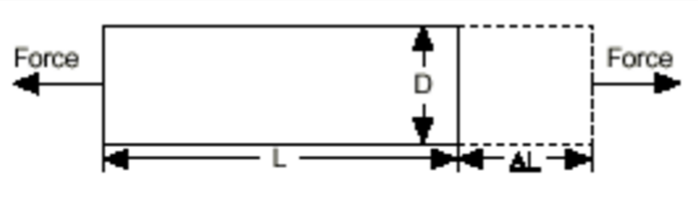
\includegraphics[scale=0.6]{figuras/fig-distension.png}
		\caption{Distension \cite{strain-def}}
		\label{fig-distension}
	\end{figure}

	Generally, the length variation in a strain gauge is very small and this makes them very susceptible to measurement errors. As a result, the use of a Wheatstone bridge is very common, it is formed by four resistive arms and an excitation voltage applied to the bridge \cite{window1982strain}.

	\begin{figure}[htbp]
		\centering
			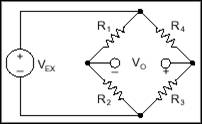
\includegraphics[scale=1.45]{figuras/fig-wheatstone.jpg}
		\caption{Wheatstone bridge \cite{wheat-bridge}}
		\label{fig-wheatstone}
	\end{figure}

	The voltage output $V_{O}$ can be obtained from the Equation \ref{eqn-voWheatstone} above:

	\begin{equation}\label{eqn-voWheatstone}
		V_{O}=\frac{ R_{3} }{ R_{3} + R_{4} } - \frac{ R_{2} }{ R_{1} + R_{2}}
	\end{equation}
